\documentclass[article]{proc}
\usepackage{abstract}
\renewcommand{\abstractname}{}    % clear the title
\renewcommand{\absnamepos}{empty} % originally center

\titleConf{DAII\\
December 13th, 2019}
\city{Austin, TX, USA}
\usepackage{color}
\usepackage{graphicx}
\begin{document}
%%%%%%%%%%%%%%%%%%%%%%%%%%%%%%%%%%%%%%%%%%%%%%%%%%%%%%%%%%%%%%%%%%%%%%%%%%%%%%%%%%%%%%%%%%%%%%%%
\title{A quantitative framework for fire department unit purchasing decisions}
%For at least  authors with different addresses, use instead the following commands
\corrauthor[1]{Tyler C. Buffington}
\corremail{tyler.c.buffington@utexas.edu}
% \doi{http://dx.doi.org/10.1615/TFESC.XXX.XXX}
\address[1]{The University of Texas at Austin, Austin, TX, 78712, USA}

\maketitle
%%%%%%%%%%%%%%%%%%%%%%%%%%%%%%%%%%%%%%%%%%%%%%%%%%%%%%%%%%%%%%%%%%%%%%%%%%%%%%%%%%%%%%%%%%%%%%%%



\section{Introduction}



\section{Decision Overview}
The purpose of this analysis is to determine the best strategy for purchasing new units for a fire department using real operational data. However, due to confidentiality issues, the identity of the department is not disclosed. 






\begin{table}[h]
\centering
\caption{An example of the resulting dataframe from the data processing described in this section. The first three minutes of May 14th are shown with minute 0 representing 12:00 AM, minute 1 representing 12:01 AM, etc. In this example, a call was placed at 12:01 AM, but not at the other minutes shown.}
\begin{tabular}{|l|l|l|l|}
\hline
\textbf{Date} & \textbf{Minute} & \textbf{Day of Week} & \textbf{Call placed?} \\ \hline
05/14/2019    & 0               & Tuesday              & 0                     \\ \hline
05/14/2019    & 1               & Tuesday              & 1                     \\ \hline
05/14/2019    & 2               & Tuesday              & 0                     \\ \hline
\end{tabular}
\label{minutedf}
\end{table}






\section{Modeling methodology}
\subsection{Data processing}
The starting point for the modeling effort described in this report is a large dataframe of incident data containing information on over 82,000 unit dispatches that occurred between May of 2015 and November of 2019. Each row of this dataframe is a dispatch of either an ALS or a suppression unit. The columns of the dataframe correspond to the unit id, the unit type, the time the unit was dispatched, the time the unit was cleared from the incident, where the incident occurred, and the station that houses the unit. Based on the location of the incident, each row also contains a \textit{first due} station entry. This entry is based on the fact that the department's jurisdictional region is divided into six smaller non-overlapping regions (one for each station) that each comprise the set of locations that are assigned to a station. Loosely speaking, the first due assignments are based on distance, meaning that for example, Station A's first due area is the set of locations that are closer to Station A than any other station. However, other factors affect these assignments and the boundaries of the first due areas are considered a ``take as given" for the purposes of this project.


The first step was to split the dataframe into two separate dataframes- one containing only ALS units and one containing only fire suppression units. Then each dataframe was grouped by the first due station corresponding to the location of the incident. For each station and each unit type, two response time arrays were generated- one corresponding to units that belong to the first due station, and one corresponding to units that came from other stations. These distribution comparisons are shown in Figure \ref{fig:alsdiff} for ALS units and fire suppression units in Figure \ref{fig:firediff}.


\begin{figure}[!htb]
  \centering
  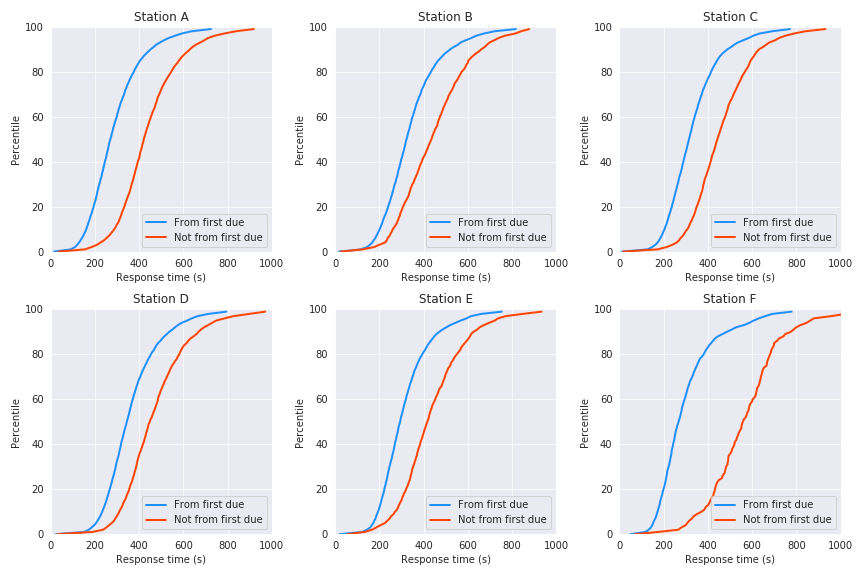
\includegraphics[width=16cm,keepaspectratio]{Figures/alsdiff.png}
  \caption{A comparison of the ALS travel time distributions between cases when the unit is from the first due area vs. when the unit is not from the first due area, broken down by each first due area.}
  \label{fig:alsdiff}
\end{figure}

\begin{figure}[!htb]
  \centering
  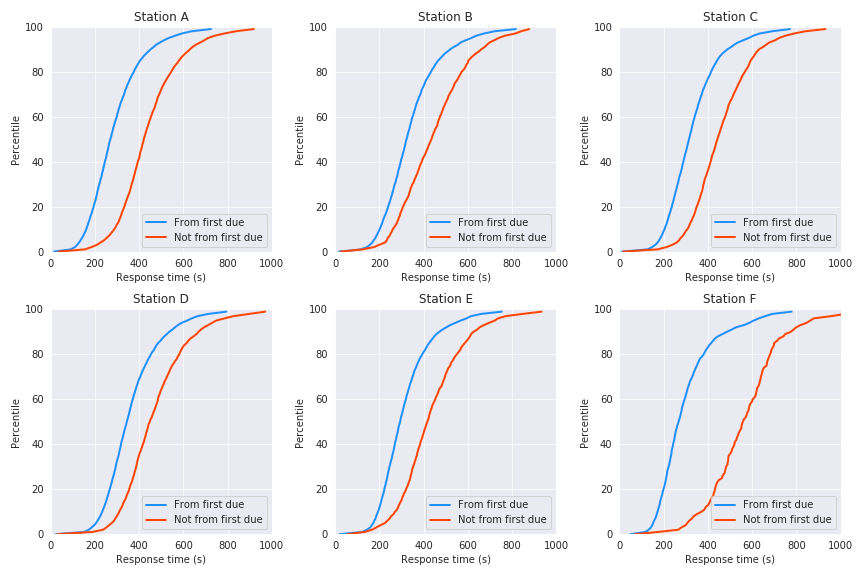
\includegraphics[width=16cm,keepaspectratio]{Figures/alsdiff.png}
  \caption{A comparison of the suppression travel time distributions between cases when the unit is from the first due area vs. when the unit is not from the first due area, broken down by each first due area.}
  \label{fig:firediff}
\end{figure}

Then, the probability of a unit being sent to an incident occurring in each first due area was calculated along with the probability that the unit was sent from the first due station. Based on these probabilities, one can imagine a simplified probability tree like the one shown in Figure \ref{fig:alstree}. 

\begin{figure}[!htb]
  \centering
  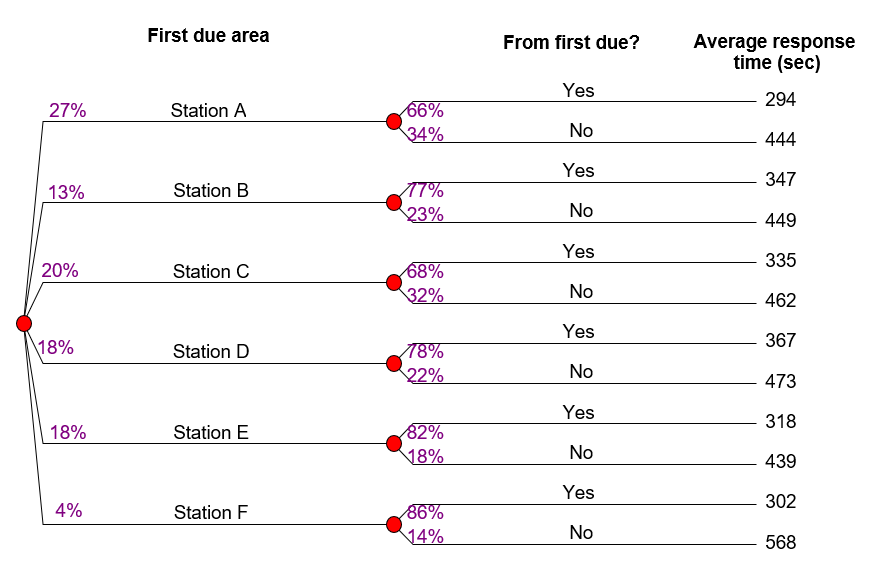
\includegraphics[width=16cm,keepaspectratio]{Figures/alstree.PNG}
  \caption{A simplified probability tree showing the main uncertainties relevant to the project. The values shown are the actual values for ALS units. Note that the average response times are shown for simplicity. In reality each of these is a distribution.}
  \label{fig:alstree}
\end{figure}

Based on the tree shown in Figure \ref{fig:alsdiff}, the effect of additional units can be modeled as a change to the ``From first due?" probability. In general, units are dispatched from non-first-due stations because the first due station does not have enough units to respond adequately. As a result, the effect of new units can be simulated by exploring the frequency of units being required in first due areas of stations while the first due station is out of units of the specified type. In order to do this, the author built an algorithm that iterates through each dataframe and determines the units of the same type that were active at the moment each unit was dispatched; active means that a unit is between its dispatched timestamp and its cleared timestamp.
As a simple example, one can imagine three hypothetical unit dispatches- Unit A, which is dispatched at 12:00 PM and cleared at 1:00 PM, Unit B, which is dispatched at 12:30 PM and cleared at 1:30 PM, and Unit C, which is dispatched at 12:45 PM and cleared at 2:00 PM. Assuming these three dispatched comprise the entire dataset, then for Unit A, the algorithm would determine that no units were active at the time Unit A was dispatched. For Unit B, it would identify that Unit A was active at the time of dispatch, and for Unit C, it would identify that both Unit A and Unit B were active at the time of dispatch. 

It is important to note that a unit can be unavailable even though it is not responding to an incident. For example, a unit can be taken out of service for maintenance, or there could be insufficient personnel to staff the unit at the moment it would be required. In order to estimate the frequency that units are unavailable for reasons such as these, we calculate the probability that a unit from a non-first-due station is dispatched instead of one from a first due station given that the unit from the first due station is not responding to a call. This probability is about 0.1 for all six first due areas. It is then assumed that






\subsection{Distribution fitting}
For this project, several different methods of estimating hypothetical response time distributions were considered. Ideally, these methods should possess three attributes. First of all, they should be accurate, meaning that they produce estimations of the response time distributions that align with reality. Next, they should be modular, meaning that they can be easily recalculated for different modeling inputs. Finally, they should be computationally inexpensive so that an optimization routine can run many iterations in a relatively short amount of time. 








The final approach to modeling the response time distributions is to utilize the observation reported by Buffington and Ezekoye \cite{buffington2019statistical} and Lu Lu et al. \cite{lu2014correlation} that fire department response times are well modeled by a log-normal distribution, meaning that the logarithm of response times are normally distributed. The assumption of normality is convenient because it allows for a unique characterization of the distribution by only calculating two parameters- a mean and a variance of the log-transformed response times. For a specified unit type, let $f_i$ be the probability that station $i$ is the first due station.  Then let $d_i$ be the probability that a unit came from station $i$ given that it is responding to an incident in the first due area of station $i$. From there, two vectors are constructed, $\alpha$ and $\beta$, each of containing six elements, where $\alpha_i = f_id_i$ and $\beta_i = f_i(1-d_i)$. Each entry in $\alpha$ is the joint probability of a unit responding to an incident in the first due area of station $i$ and that unit is from station $i$; conversely, each entry in $\beta$ is the joint probability of a unit responding to an incident in the first due area of station $i$ and that unit is \textit{not} from station $i$. These two vectors can be concatenated into a single vector, $w = [\alpha, \beta]^T$, of length 12, corresponding to the 12 response time distributions shown in Figure \ref{fig:alsdiff} or Figure \ref{fig:firediff}, depending on the unit type. The probability of a draw from the $j^{th}$ conditional response time distribution is therefore $w_j$. Next, the estimated mean, $\hat\mu \in R$, and the estimated variance, $\hat\sigma^2 \in R$ of the marginal log-transformed response time distribution are calculated. The calculation of the mean is relatively straightforward and is shown in Equation \ref{eq:mean_calc},


\begin{equation}
\hat\mu = w^Tm
\label{eq:mean_calc}
\end{equation}


where $m \in R^{12}$ contains the means of the log-transformed response times, which are calculated according to Equation \ref{eq:mean}:

\begin{equation}
m_j = \frac{1}{N_j}\sum_{k=1}^{N_j}log(t_{j,k})
\label{eq:mean}
\end{equation}


where $N_j$ is the number of dispatches that satisfy condition $j$, and $t_j$ is the set of reported response times corresponding to these dispatches.


In order to calculate $\hat\sigma^2$, the following variance relation is employed:


\begin{equation}
\hat\sigma^2 = \underbrace{E\big[log(t)^2\big]}_{I} - \underbrace{\bigg(E\big[log(t)\big]\bigg)^2}_{II}
\label{eq:var}
\end{equation}

Term I is then calculated according to Equation \ref{eq:mean_sq_calc}:

\begin{equation}
E\big[log(t)^2\big] = w^Tm'
\label{eq:mean_sq_calc}
\end{equation}

where 
$m'_j = \frac{1}{N_j}\sum_{k=1}^{N_j}log(t_{j,k})^2$. Term II is just the square of the mean calculated in Equation \ref{eq:mean_calc}, i.e. $\big(E\big[log(t)\big]\big)^2 = \hat\mu^2$. Once $\hat\mu$ and $\hat\sigma^2$ are calculated, they are then used to characterize a normal distribution (i.e. $ log(t) \sim N(\hat\mu, \hat\sigma^2)$), and the resulting log-normal distribution is determined by exponentiating this distribution. The cdf of the resulting log-normal distribution is shown alongside the empirical cdf for all of the reported response times in the dataset in Figure 


\begin{figure}[!htb]
  \centering
  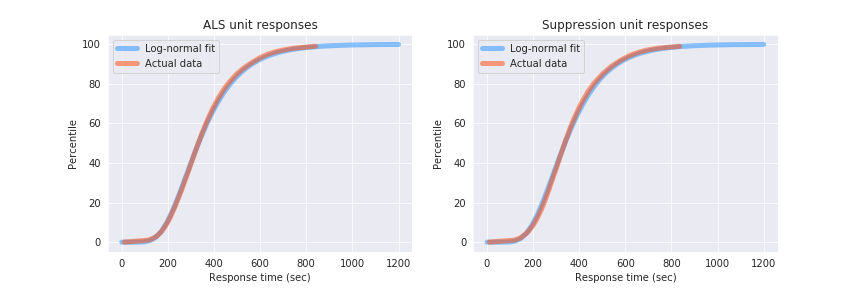
\includegraphics[width=16cm,keepaspectratio]{Figures/lognorm.png}
  \caption{}
  \label{fig:alstree}
\end{figure}






\subsection{Optimization}



\section{Insights and recommendations}


\section{Conclusions and future work}




\bibliographystyle{Bibliography_Style}
\scriptsize{
\bibliography{./References}
}

\end{document}
